\documentclass[10pt,a4paper]{article}

% -----------------------------------------------------------------------------
% MATHS MANTHAN | Class 10 Pair of Linear Equations in Two Variables | 2026--27
% Self-contained publication-quality master formula & concept handbook.
% Strictly compliant with the rationalized CBSE Class 10 curriculum.
% Exactly 14 Pages with zero overfull boxes or unintended page overflow.
% -----------------------------------------------------------------------------

\usepackage[a4paper,top=12mm,bottom=15mm,left=15mm,right=15mm,footskip=8mm]{geometry}
\usepackage[T1]{fontenc}
\usepackage{lmodern}
\usepackage{microtype}
\usepackage{amsmath,amssymb}
\usepackage[table]{xcolor}
\usepackage{array,tabularx,booktabs}
\usepackage{graphicx}
\usepackage{eso-pic}
\usepackage{tikz}
\usetikzlibrary{calc,positioning,arrows.meta,shapes.geometric,patterns}
\usepackage[most]{tcolorbox}
\usepackage{enumitem}
\usepackage{fancyhdr}
\usepackage{lastpage}
\usepackage[hidelinks]{hyperref}
\usepackage{url}

% Compatibility fix for modern LaTeX/MiKTeX: colortbl + tabularx p-column alignment
\makeatletter
\let\insert@pcolumn\insert@column
\makeatother

% ============================================================================
% BRAND COLOR PALETTE — MATCHED TO THE MATHS MANTHAN STANDARD
% Primary navy: #001F49 | Brand gold: #D19029
% ============================================================================
\definecolor{primary}{RGB}{0,31,73}
\definecolor{brandnavy}{RGB}{0,31,73}
\definecolor{accent}{RGB}{209,144,41}
\definecolor{brandgold}{RGB}{209,144,41}
\definecolor{secondary}{RGB}{75,85,99}
\definecolor{lightgray}{RGB}{246,248,250}
\definecolor{accentlight}{RGB}{254,250,242}
\definecolor{primarylight}{RGB}{240,244,250}

\colorlet{navy}{primary}
\colorlet{blue}{primary!82!black}
\colorlet{gold}{accent}
\colorlet{goldpale}{accentlight}
\colorlet{bluepale}{primarylight}
\colorlet{ink}{secondary}
\colorlet{muted}{secondary}
\colorlet{linegray}{primary!25}
\colorlet{reddeep}{primary}
\colorlet{redpale}{lightgray}
\colorlet{green}{primary}
\colorlet{greenpale}{primarylight}

% Automatic low-opacity logo watermark on every page
\IfFileExists{mathsmanthan logo.png}{%
  \AddToShipoutPictureBG{%
    \begin{tikzpicture}[remember picture,overlay]
      \node[opacity=0.065] at (current page.center) {%
        \includegraphics[width=0.55\paperwidth,keepaspectratio]{mathsmanthan logo.png}%
      };
    \end{tikzpicture}%
  }%
}{}

\hypersetup{
  pdftitle={Class 10 Pair of Linear Equations | Maths Manthan Handbook},
  pdfauthor={Maths Manthan Tuition Classes},
  pdfsubject={CBSE Class 10 Mathematics, Academic Year 2026--27},
  pdfkeywords={Pair of Linear Equations in Two Variables, Substitution, Elimination, Consistency, CBSE Class 10, Maths Manthan}
}

\setlength{\parindent}{0pt}
\setlength{\parskip}{2pt}
\renewcommand{\arraystretch}{1.15}
\setlist[itemize]{leftmargin=4.5mm,itemsep=1pt,topsep=1pt,parsep=0pt}
\setlist[enumerate]{leftmargin=5.5mm,itemsep=1pt,topsep=1pt,parsep=0pt}
\setlength{\tabcolsep}{4.5pt}
\emergencystretch=2em
\hfuzz=1pt

% ============================================================================
% HEADER / FOOTER
% ============================================================================
\newcommand{\TuitionName}{{\color{primary}MATHS} {\color{accent}MANTHAN}}
\newcommand{\TuitionSub}{{\color{primary}\textbullet\ \ \text{TUITION CLASSES}\ \ \textbullet}}
\newcommand{\ContactInfo}{e-mail: contact@mathsmanthan.co.in \quad$\vert$\quad Helpline: +91-8171546558}
\newcommand{\HandbookFooterTitle}{Class 10 Pair of Linear Equations Handbook}

\pagestyle{fancy}
\fancyhf{}
\renewcommand{\headrulewidth}{0pt}
\renewcommand{\footrulewidth}{0.6pt}
\renewcommand{\footrule}{\hbox to\headwidth{\color{primary!30}\leaders\hrule height 0.6pt\hfill}}
\fancyfoot[L]{\footnotesize\href{https://mathsmanthan.co.in}{\textcolor{secondary}{\TuitionName\ $\vert$\ \HandbookFooterTitle}}}
\fancyfoot[R]{\footnotesize\textbf{\color{primary}Page \thepage\ of \pageref{LastPage}}\quad\textcolor{accent}{\textbf{Academic Year 2026--27}}}

\fancypagestyle{plain}{%
  \fancyhf{}
  \fancyfoot[L]{\footnotesize\href{https://mathsmanthan.co.in}{\textcolor{secondary}{\TuitionName\ $\vert$\ \HandbookFooterTitle}}}
  \fancyfoot[R]{\footnotesize\textbf{\color{primary}Page \thepage\ of \pageref{LastPage}}\quad\textcolor{accent}{\textbf{Academic Year 2026--27}}}
  \renewcommand{\headrulewidth}{0pt}
  \renewcommand{\footrulewidth}{0.6pt}
  \renewcommand{\footrule}{\hbox to\headwidth{\color{primary!30}\leaders\hrule height 0.6pt\hfill}}
}

% Reusable design components
\newcommand{\BrandMark}{%
  \IfFileExists{mathsmanthan logo.png}{%
    \includegraphics[width=22mm,height=22mm,keepaspectratio]{mathsmanthan logo.png}%
  }{%
    
\begin{tikzpicture}[baseline=-0.6ex]
      \fill[navy,rounded corners=2.2pt] (0,0) rectangle (1.45,1.05);
      \draw[gold,line width=1.2pt] (0.15,0.15)--(1.30,0.15);
      \node[text=white,font=\sffamily\bfseries\Large] at (0.725,0.59) {MM};
    \end{tikzpicture}%
  }%
}

\newcommand{\chapterbanner}[4]{%
  \begin{tcolorbox}[enhanced,colback=bluepale,colframe=bluepale,boxrule=0pt,arc=2mm,
    left=3.5mm,right=3.5mm,top=1.8mm,bottom=1.8mm]
    {\footnotesize\bfseries\color{gold}CHAPTER #1\hfill\color{blue}#4}\par\vspace{0.4mm}
    {\Large\bfseries\color{navy}#2}\par
    {\small\color{muted}#3}
  \end{tcolorbox}\vspace{0.8mm}
}

\newcommand{\subhead}[1]{%
  \vspace{1mm}{\large\bfseries\color{navy}#1}\par\vspace{0.3mm}
  {\color{gold}\rule{14mm}{1.2pt}}\par\vspace{0.8mm}
}

\newtcolorbox{formulaBox}[1][]{enhanced,breakable,colback=goldpale,colframe=gold!65!black,
  boxrule=0.5pt,arc=1.5mm,left=2.8mm,right=2.8mm,top=1.8mm,bottom=1.8mm,
  before skip=2pt,after skip=3pt,#1}
\newtcolorbox{conceptBox}[1][]{enhanced,breakable,colback=bluepale,colframe=blue!25,
  boxrule=0.4pt,arc=1.5mm,left=2.8mm,right=2.8mm,top=1.8mm,bottom=1.8mm,
  before skip=2pt,after skip=3pt,#1}
\newtcolorbox{warningBox}[1][]{enhanced,breakable,colback=redpale,colframe=reddeep!45,
  boxrule=0.45pt,arc=1.5mm,left=2.8mm,right=2.8mm,top=1.8mm,bottom=1.8mm,
  before skip=2pt,after skip=3pt,#1}
\newtcolorbox{successBox}[1][]{enhanced,breakable,colback=greenpale,colframe=green!35,
  boxrule=0.45pt,arc=1.5mm,left=2.8mm,right=2.8mm,top=1.8mm,bottom=1.8mm,
  before skip=2pt,after skip=3pt,#1}

\newcommand{\CoreTag}{\tcbox[colback=greenpale,colframe=green!40,boxrule=.3pt,arc=1mm,left=1.5mm,right=1.5mm,top=.5mm,bottom=.5mm]{\scriptsize\bfseries\color{green}CORE SYLLABUS}}
\newcommand{\ExamTag}{\tcbox[colback=bluepale,colframe=blue!25,boxrule=.3pt,arc=1mm,left=1.5mm,right=1.5mm,top=.5mm,bottom=.5mm]{\scriptsize\bfseries\color{blue}EXAM STRATEGY}}
\newcommand{\TrapTag}{\tcbox[colback=redpale,colframe=reddeep!40,boxrule=.3pt,arc=1mm,left=1.5mm,right=1.5mm,top=.5mm,bottom=.5mm]{\scriptsize\bfseries\color{reddeep}TRAP ALERT}}
\newcommand{\ReferenceTag}{\tcbox[colback=bluepale,colframe=blue!25,boxrule=.3pt,arc=1mm,left=1.5mm,right=1.5mm,top=.5mm,bottom=.5mm]{\scriptsize\bfseries\color{blue}QUICK REFERENCE}}

\begin{document}

% =============================================================================
% PAGE 1: STANDALONE INSTITUTIONAL COVER PAGE
% =============================================================================
\thispagestyle{fancy}
\vspace*{0mm}
\noindent
\makebox[0pt][l]{%
  \raisebox{-0.80cm}[0pt][0pt]{%
    \href{https://mathsmanthan.co.in}{\BrandMark}%
  }%
}%
\parbox{\textwidth}{%
  \centering
  \href{https://mathsmanthan.co.in}{%
    {\fontsize{23pt}{23pt}\selectfont\bfseries \TuitionName}\\[3pt]
    {\footnotesize\bfseries \TuitionSub}%
  }\\[2pt]
  {\scriptsize\color{secondary} \ContactInfo}
}

\vspace{4pt}
\noindent{\color{primary}\rule{0.72\textwidth}{1.5pt}}\hfill{\color{accent}\rule{0.26\textwidth}{1.5pt}}

\vspace{3mm}
\begin{center}
  {\large\bfseries\color{muted}CBSE CLASS 10 \;$\vert$\; MATHEMATICS}\\[3mm]
  {\fontsize{24}{28}\selectfont\bfseries\color{navy}PAIR OF LINEAR EQUATIONS IN TWO VARIABLES}\\[2mm]
  {\Large\color{blue}Master Concept, Formula \& Visual Problem-Solving Handbook}\\[2mm]
  {\large\color{gold}\bfseries Academic Year 2026--27}
\end{center}

\vspace{2.5mm}

\begin{tikzpicture}
  \fill[navy,rounded corners=3mm] (0,0) rectangle (\textwidth,2.8);
  \draw[gold,line width=2pt] (0.35,0.35)--(0.35,2.45);
  \node[anchor=west,text=white,font=\bfseries\Large] at (0.7,2.2) {Plot the constraints. Compare the ratios.};
  \node[anchor=west,text=white,font=\Large] at (0.7,1.7) {Solve with absolute precision.};
  \node[anchor=west,text=white,font=\small] at (0.7,1.1) {Geometric Tri-State \;$\vert$\; Graphical Intersections \;$\vert$\; Substitution \;$\vert$\; Elimination \;$\vert$\; Word Models};
  \node[anchor=west,text=white!75,font=\footnotesize] at (0.7,0.55) {A student-first Maths Manthan conceptual and visual revision resource};
  \foreach \x/\r in {14.7/0.85,14.7/0.56,14.7/0.28} {\draw[gold!80,line width=1.1pt] (\x,1.4) circle (\r);}
  \fill[gold] (14.7,1.4) circle (0.08);
\end{tikzpicture}

\vspace{3mm}
\begin{minipage}[t]{0.48\textwidth}
  \begin{conceptBox}[title=What This Handbook Includes,fonttitle=\bfseries\color{navy}]
    \begin{itemize}
      \item Standard form criteria and geometry of simultaneous lines
      \item The Tri-State system: intersecting, coincident, and parallel
      \item Graphical solutions and coordinates of enclosed triangles
      \item Algebraic solving: Substitution and Elimination workflows
      \item The high-speed Symmetric Coefficients addition shortcut
      \item Parameter $k$ consistency protocols and real-world models
    \end{itemize}
  \end{conceptBox}
\end{minipage}\hfill
\begin{minipage}[t]{0.48\textwidth}
  \begin{formulaBox}[title=Pedagogical Strategy: Foundations First,fonttitle=\bfseries\color{navy}]
    \raggedright A linear equation in two variables represents an infinite locus of collinear points. A simultaneous system represents intersecting constraints:
    \begin{center}
      \small\textbf{\color{navy}Unique Solution $(x_0, y_0) \iff$ Intersecting Lines}\\[2pt]
      \small\textbf{\color{navy}Ratio Test: $\frac{a_1}{a_2} \neq \frac{b_1}{b_2} \iff$ Distinct Slopes}
    \end{center}
    Always inspect the coefficient ratios before deciding the solving technique!
  \end{formulaBox}
\end{minipage}

\vspace{1.5mm}
\begin{warningBox}[title=CBSE 2026--27 Curriculum Verification \& Rationalized Scope,fonttitle=\bfseries\color{navy}]
  \textbf{Official Scope (Prescribed \& Tested):} Pair of linear equations in two variables and graphical method of their solution, consistency/inconsistency. Algebraic conditions for number of solutions. Solution by Substitution and by Elimination. Situational word problems.\\
  \textbf{Excluded / Deleted Topics (Non-Examinable):}
  \begin{itemize}
    \item \textbf{Cross-Multiplication Method:} Completely deleted from the NCERT syllabus.
    \item \textbf{Equations Reducible to Linear Form:} Systems requiring $u = \frac{1}{x}, v = \frac{1}{y}$ substitutions are deleted.
  \end{itemize}
\end{warningBox}

\vfill
\begin{center}
  {\small\bfseries\color{navy}Maths Manthan Tuition Classes}\\
  {\footnotesize\color{muted}contact@mathsmanthan.co.in \quad$\vert$\quad +91-8171546558}\\
  {\footnotesize\url{https://mathsmanthan.co.in}}\\[1.5mm]
  {\scriptsize\color{muted}Prepared for learning and conceptual mastery \;--\; Strictly aligned with CBSE Class 10 Syllabus 2026--27.}
\end{center}

\newpage

% =============================================================================
% PAGE 2: MODULE 1 — STANDARD FORM & CARTESIAN FOUNDATIONS
% =============================================================================
\thispagestyle{fancy}
\vspace*{0mm}

\chapterbanner{03}{PAIR OF LINEAR EQUATIONS IN TWO VARIABLES}{Module 1 $\vert$ Foundations: Standard Form \& Cartesian Geometry}{\CoreTag}

\subhead{1.1 Definition and General Form of a Linear Equation}

An equation which can be put in the form $\mathbf{ax + by + c = 0}$, where $a, b, c \in \mathbb{R}$ and $a, b$ are not both zero ($a^2 + b^2 \neq 0$), is called a \textbf{linear equation in two variables} $x$ and $y$.

\begin{minipage}[c]{0.52\textwidth}
\begin{formulaBox}
  \textbf{General Form of a Pair of Linear Equations:}
  $$\mathbf{a_1 x + b_1 y + c_1 = 0}$$
  $$\mathbf{a_2 x + b_2 y + c_2 = 0}$$
  where $a_1^2 + b_1^2 \neq 0$ and $a_2^2 + b_2^2 \neq 0$.
  \begin{itemize}
    \item \textbf{Geometric Representation:} Every linear equation in two variables represents a \textbf{straight line} on the Cartesian plane.
    \item \textbf{Meaning of Solution:} An ordered pair $(x_0, y_0)$ is a \textbf{solution} of the system if and only if it satisfies both equations simultaneously.
    \item Geometrically, $(x_0, y_0)$ is the \textbf{common point} lying on both lines!
  \end{itemize}
\end{formulaBox}
\end{minipage}\hfill
\begin{minipage}[c]{0.45\textwidth}
\centering
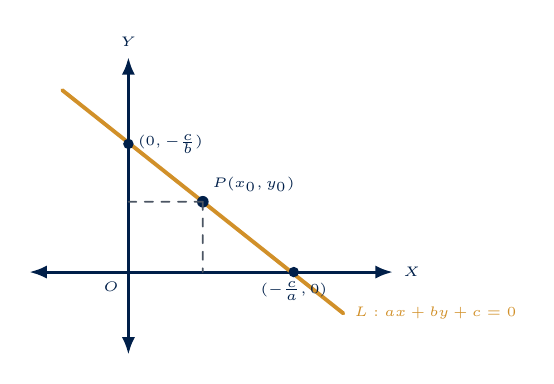
\begin{tikzpicture}[scale=1.05, line cap=round, line join=round]
  % Axes
  \draw[{Latex[scale=0.8]}-{Latex[scale=0.8]}, primary, line width=1.1pt] (-1.2,0) -- (3.2,0) node[right, font=\tiny\bfseries]{$X$};
  \draw[{Latex[scale=0.8]}-{Latex[scale=0.8]}, primary, line width=1.1pt] (0,-1.0) -- (0,2.6) node[above, font=\tiny\bfseries]{$Y$};
  \node[font=\tiny\bfseries\color{navy}, below left] at (0,0) {$O$};

  % Line ax + by + c = 0
  \draw[accent, line width=1.4pt] (-0.8,2.2) -- (2.6,-0.5) node[right, font=\tiny\bfseries\color{accent}]{$L: ax+by+c=0$};

  % Intercepts
  \fill[reddeep] (0,1.55) circle (1.8pt) node[right, font=\tiny\bfseries\color{reddeep}]{$(0, -\frac{c}{b})$};
  \fill[reddeep] (2.0,0) circle (1.8pt) node[below, font=\tiny\bfseries\color{reddeep}]{$(-\frac{c}{a}, 0)$};

  % Solution point P
  \coordinate (P) at (0.9,0.85);
  \fill[primary] (P) circle (2pt) node[above right, font=\tiny\bfseries\color{navy}]{$P(x_0, y_0)$};
  \draw[dashed, secondary, line width=0.6pt] (P) -- (0.9,0);
  \draw[dashed, secondary, line width=0.6pt] (P) -- (0,0.85);
\end{tikzpicture}
\end{minipage}

\vspace{0.8mm}
\subhead{1.2 Verifying Whether an Ordered Pair is a Solution}

To test whether a given point $(x_0, y_0)$ is a solution of a system, substitute $x = x_0$ and $y = y_0$ into \textbf{both equations}. If both LHS equal RHS, the point is a solution; if it fails in even one equation, it is \textbf{not} a solution.

\vspace{0.8mm}
\begin{conceptBox}[title={Worked Archetype 1 $\vert$ Algebraic Solution Verification},fonttitle=\bfseries\color{navy}]
  \textbf{Problem:} Check whether $x = 3, y = 2$ and $x = 1, y = 4$ are solutions of the system:
  $$2x + 3y = 12 \qquad \text{and} \qquad x - 2y = -1$$
  \par\vspace{0.6mm}\noindent
  \textbf{Check for $(3, 2)$:}
  \begin{itemize}
    \item Equation 1: $\text{LHS} = 2(3) + 3(2) = 6 + 6 = 12 = \text{RHS}$. (Satisfied!)
    \item Equation 2: $\text{LHS} = 3 - 2(2) = 3 - 4 = -1 = \text{RHS}$. (Satisfied!)
  \end{itemize}
  Since $(3, 2)$ satisfies both equations, $\mathbf{(3, 2) \text{ IS a solution}}$ of the system.
  \par\noindent
  \textbf{Check for $(1, 4)$:}
  \begin{itemize}
    \item Equation 1: $\text{LHS} = 2(1) + 3(4) = 2 + 12 = 14 \neq 12$.
  \end{itemize}
  Since $(1, 4)$ fails in Equation 1, $\mathbf{(1, 4) \text{ is NOT a solution}}$.
\end{conceptBox}

\newpage

% =============================================================================
% PAGE 3: MODULE 2 — THE TRI-STATE GEOMETRIC SYSTEM
% =============================================================================
\thispagestyle{fancy}
\vspace*{0mm}

\chapterbanner{03}{PAIR OF LINEAR EQUATIONS IN TWO VARIABLES}{Module 2 $\vert$ The Tri-State Geometric System: Intersecting, Coincident \& Parallel Lines}{\CoreTag}

\subhead{2.1 The Three Geometrical Configurations of Two Lines in a Plane}

Two straight lines $L_1$ and $L_2$ drawn on the Cartesian plane can exhibit exactly one of three spatial relationships:

\begin{center}
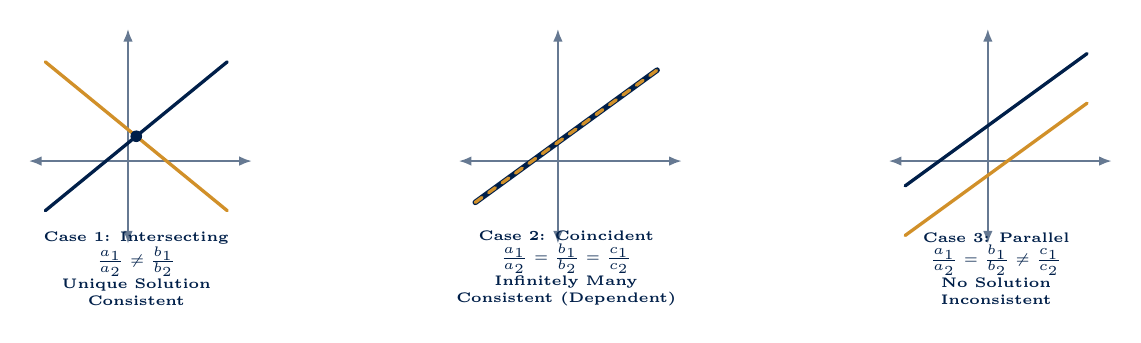
\begin{tikzpicture}[scale=1.05, line cap=round, line join=round]
  % Case 1: Intersecting
  \begin{scope}[shift={(0,0)}]
    \draw[{Latex[scale=0.7]}-{Latex[scale=0.7]}, primary!60, line width=0.8pt] (-1.2,0) -- (1.5,0);
    \draw[{Latex[scale=0.7]}-{Latex[scale=0.7]}, primary!60, line width=0.8pt] (0,-1.0) -- (0,1.6);
    \draw[primary, line width=1.2pt] (-1.0,-0.6) -- (1.2,1.2);
    \draw[accent, line width=1.2pt] (-1.0,1.2) -- (1.2,-0.6);
    \fill[reddeep] (0.1,0.3) circle (2pt);
    \node[font=\tiny\bfseries\color{navy}, align=center] at (0.1,-1.3) {\textbf{Case 1: Intersecting}\\$\frac{a_1}{a_2} \neq \frac{b_1}{b_2}$\\\textbf{Unique Solution}\\\textbf{Consistent}};
  \end{scope}

  % Case 2: Coincident
  \begin{scope}[shift={(5.2,0)}]
    \draw[{Latex[scale=0.7]}-{Latex[scale=0.7]}, primary!60, line width=0.8pt] (-1.2,0) -- (1.5,0);
    \draw[{Latex[scale=0.7]}-{Latex[scale=0.7]}, primary!60, line width=0.8pt] (0,-1.0) -- (0,1.6);
    \draw[primary, line width=2pt] (-1.0,-0.5) -- (1.2,1.1);
    \draw[accent, dashed, line width=1.2pt] (-1.0,-0.5) -- (1.2,1.1);
    \node[font=\tiny\bfseries\color{navy}, align=center] at (0.1,-1.3) {\textbf{Case 2: Coincident}\\$\frac{a_1}{a_2} = \frac{b_1}{b_2} = \frac{c_1}{c_2}$\\\textbf{Infinitely Many}\\\textbf{Consistent (Dependent)}};
  \end{scope}

  % Case 3: Parallel
  \begin{scope}[shift={(10.4,0)}]
    \draw[{Latex[scale=0.7]}-{Latex[scale=0.7]}, primary!60, line width=0.8pt] (-1.2,0) -- (1.5,0);
    \draw[{Latex[scale=0.7]}-{Latex[scale=0.7]}, primary!60, line width=0.8pt] (0,-1.0) -- (0,1.6);
    \draw[primary, line width=1.2pt] (-1.0,-0.3) -- (1.2,1.3);
    \draw[accent, line width=1.2pt] (-1.0,-0.9) -- (1.2,0.7);
    \node[font=\tiny\bfseries\color{navy}, align=center] at (0.1,-1.3) {\textbf{Case 3: Parallel}\\$\frac{a_1}{a_2} = \frac{b_1}{b_2} \neq \frac{c_1}{c_2}$\\\textbf{No Solution}\\\textbf{Inconsistent}};
  \end{scope}
\end{tikzpicture}
\end{center}

\vspace{0.8mm}
\subhead{2.2 The Master Ratio Comparison Table}

Let $a_1 x + b_1 y + c_1 = 0$ and $a_2 x + b_2 y + c_2 = 0$ be the system in standard form:

\begin{center}
\small
\begin{tabularx}{\textwidth}{c p{36mm} p{34mm} X}
\toprule
\rowcolor{bluepale}
\textbf{Ratio Comparison} & \textbf{Graphical Representation} & \textbf{Algebraic Solutions} & \textbf{System Consistency Status} \\
\midrule
$\mathbf{\frac{a_1}{a_2} \neq \frac{b_1}{b_2}}$ & Intersecting lines & Exactly \textbf{one unique solution} & \textbf{Consistent} (system has a solution). \\
\rowcolor{lightgray}
$\mathbf{\frac{a_1}{a_2} = \frac{b_1}{b_2} = \frac{c_1}{c_2}}$ & Coincident (overlapping) lines & \textbf{Infinitely many solutions} & \textbf{Consistent (Dependent)}. \\
$\mathbf{\frac{a_1}{a_2} = \frac{b_1}{b_2} \neq \frac{c_1}{c_2}}$ & Parallel (non-intersecting) lines & \textbf{No solution} & \textbf{Inconsistent} (no common point). \\
\bottomrule
\end{tabularx}
\end{center}

\vspace{0.5mm}
\begin{conceptBox}[title={Worked Archetype 2 $\vert$ Testing Consistency via Ratio Inspection},fonttitle=\bfseries\color{navy}]
  \textbf{Problem:} On comparing the ratios $\frac{a_1}{a_2}, \frac{b_1}{b_2}$, and $\frac{c_1}{c_2}$, determine whether the following pair of linear equations is consistent or inconsistent:
  $$\frac{3}{2}x + \frac{5}{3}y = 7 \qquad \text{and} \qquad 9x - 10y = 14$$
  \par\vspace{0.6mm}\noindent
  \textbf{Step 1: Write both equations in standard form $ax + by + c = 0$:}
  $$\frac{3}{2}x + \frac{5}{3}y - 7 = 0 \implies a_1 = \frac{3}{2}, \quad b_1 = \frac{5}{3}, \quad c_1 = -7$$
  $$9x - 10y - 14 = 0 \implies a_2 = 9, \quad b_2 = -10, \quad c_2 = -14$$
  \textbf{Step 2: Compute individual ratios:}
  $$\frac{a_1}{a_2} = \frac{3/2}{9} = \frac{3}{18} = \mathbf{\frac{1}{6}}, \qquad \frac{b_1}{b_2} = \frac{5/3}{-10} = \frac{5}{-30} = \mathbf{-\frac{1}{6}}$$
  \textbf{Step 3: Compare ratios:} Since $\frac{1}{6} \neq -\frac{1}{6} \implies \mathbf{\frac{a_1}{a_2} \neq \frac{b_1}{b_2}}$.\\
  \textbf{Conclusion:} The lines intersect at a unique point. Hence, the system is \textbf{consistent}.
\end{conceptBox}

\newpage

% =============================================================================
% PAGE 4: MODULE 3 — GRAPHICAL METHOD & BOUNDED TRIANGLES
% =============================================================================
\thispagestyle{fancy}
\vspace*{0mm}

\chapterbanner{03}{PAIR OF LINEAR EQUATIONS IN TWO VARIABLES}{Module 3 $\vert$ The Graphical Solution Method \& Bounded Triangular Regions}{\CoreTag}

\subhead{3.1 The 4-Step Graphical Solution Protocol}

To solve a system graphically:
\begin{enumerate}
  \item Express $y$ in terms of $x$ for each equation: $y = \frac{-a_1 x - c_1}{b_1}$.
  \item Create a table of at least two (preferably three) integer solution pairs $(x, y)$ for each line.
  \item Plot the coordinates on a uniform scale and draw straight lines extending across both axes.
  \item The coordinates $(x, y)$ of the point where the lines intersect give the unique solution!
\end{enumerate}

\begin{minipage}[c]{0.45\textwidth}
\centering
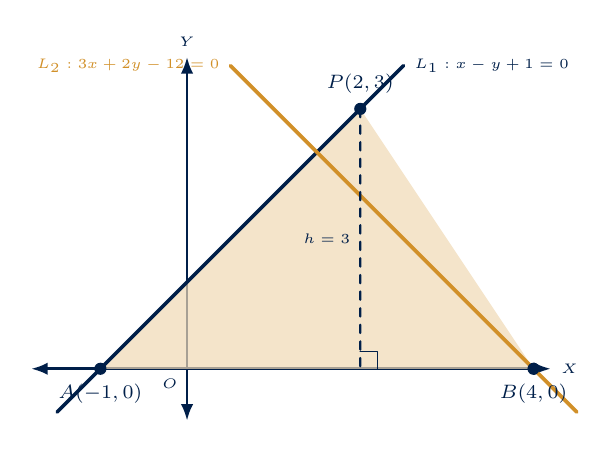
\begin{tikzpicture}[scale=1.1, line cap=round, line join=round]
  % Axes
  \draw[{Latex[scale=0.8]}-{Latex[scale=0.8]}, primary, line width=1pt] (-1.8,0) -- (4.2,0) node[right, font=\tiny\bfseries]{$X$};
  \draw[{Latex[scale=0.8]}-{Latex[scale=0.8]}, primary, line width=1pt] (0,-0.6) -- (0,3.6) node[above, font=\tiny\bfseries]{$Y$};
  \node[font=\tiny\bfseries\color{navy}, below left] at (0,0) {$O$};

  % Coordinates of triangle
  \coordinate (A) at (-1.0,0);
  \coordinate (B) at (4.0,0);
  \coordinate (P) at (2.0,3.0);

  % Shaded Triangle Region
  \fill[accent!35, opacity=0.7] (A) -- (B) -- (P) -- cycle;
  \draw[primary, line width=1.3pt] (-1.5,-0.5) -- (2.5,3.5) node[right, font=\tiny\bfseries]{$L_1: x - y + 1 = 0$};
  \draw[accent, line width=1.3pt] (4.5,-0.5) -- (0.5,3.5) node[left, font=\tiny\bfseries]{$L_2: 3x + 2y - 12 = 0$};

  % Vertices
  \fill[reddeep] (P) circle (2pt) node[above=2pt, font=\scriptsize\bfseries\color{reddeep}]{$P(2, 3)$};
  \fill[primary] (A) circle (2pt) node[below=2pt, font=\scriptsize\bfseries\color{navy}]{$A(-1, 0)$};
  \fill[primary] (B) circle (2pt) node[below=2pt, font=\scriptsize\bfseries\color{navy}]{$B(4, 0)$};

  % Altitude
  \draw[dashed, reddeep, line width=0.8pt] (P) -- (2.0,0) node[midway, left, font=\tiny\bfseries]{$h = 3$};
  \draw[reddeep, line width=0.6pt] (2.0,0.2) -- (2.2,0.2) -- (2.2,0);
\end{tikzpicture}
\end{minipage}\hfill
\begin{minipage}[c]{0.53\textwidth}
\begin{formulaBox}
  \textbf{Area of the Bounded Triangle Region:}
  When lines intersect each other at $P(x_0, y_0)$ and intersect the $x$-axis at $A(x_1, 0)$ and $B(x_2, 0)$:
  \begin{itemize}
    \item \textbf{Base of Triangle ($AB$):}
      $$\mathbf{\text{Base} = |x_2 - x_1|}$$
    \item \textbf{Height of Triangle ($h$):} The vertical distance from apex $P$ to the $x$-axis:
      $$\mathbf{h = |y_0|}$$
    \item \textbf{Enclosed Triangle Area:}
      $$\mathbf{\text{Area} = \frac{1}{2} \times \text{Base} \times \text{Height} = \frac{1}{2} \cdot |x_2 - x_1| \cdot |y_0|}$$
  \end{itemize}
\end{formulaBox}
\end{minipage}

\vspace{0.8mm}
\begin{conceptBox}[title={Worked Archetype 3 $\vert$ Graphing Lines and Shading the Enclosed Triangle},fonttitle=\bfseries\color{navy}]
  \textbf{Problem:} Draw the graphs of $x - y + 1 = 0$ and $3x + 2y - 12 = 0$. Determine the coordinates of the vertices of the triangle formed by these lines and the $x$-axis, and calculate its area.
  \par\vspace{0.6mm}\noindent
  \textbf{Step 1: Solution table for $L_1: y = x + 1$:} Points: $(-1, 0), \; (0, 1), \; (2, 3)$.\\
  \textbf{Step 2: Solution table for $L_2: y = \frac{12 - 3x}{2}$:} Points: $(0, 6), \; (2, 3), \; (4, 0)$.\\
  \textbf{Step 3: Point of Intersection:} Both tables contain the common point $\mathbf{P(2, 3)}$. Hence, $x = 2, y = 3$.\\
  \textbf{Step 4: Intersections with $x$-axis ($y = 0$):}
  \begin{itemize}
    \item For $L_1$: $x - 0 + 1 = 0 \implies x = -1 \implies \mathbf{A(-1, 0)}$.
    \item For $L_2$: $3x + 2(0) - 12 = 0 \implies 3x = 12 \implies x = 4 \implies \mathbf{B(4, 0)}$.
  \end{itemize}
  \textbf{Vertices of the Triangle:} $\mathbf{A(-1, 0), \; B(4, 0), \; P(2, 3)}$.\\
  \textbf{Area Calculation:} $\text{Base } AB = 4 - (-1) = 5\text{ units}$. $\text{Height } h = 3\text{ units}$.
  $$\mathbf{\text{Area}(\triangle PAB)} = \frac{1}{2} \times \text{base} \times \text{height} = \frac{1}{2} \times 5 \times 3 = \mathbf{7.5\text{ sq. units.}}$$
\end{conceptBox}

\newpage

% =============================================================================
% PAGE 5: MODULE 4 — ALGEBRAIC METHOD I: SUBSTITUTION
% =============================================================================
\thispagestyle{fancy}
\vspace*{0mm}

\chapterbanner{03}{PAIR OF LINEAR EQUATIONS IN TWO VARIABLES}{Module 4 $\vert$ Algebraic Method I: The Method of Substitution}{\CoreTag}

\subhead{4.1 Theoretical Mechanism of Substitution}

The **Method of Substitution** operates by using one constraint to express one variable strictly in terms of the other, thereby reducing a 2-variable simultaneous system into a **single-variable linear equation**.

\begin{center}

\begin{tikzpicture}[scale=0.95, line cap=round, line join=round]
  % Step 1
  \node[draw=primary, fill=primarylight, rounded corners=2mm, line width=1pt, font=\scriptsize\bfseries\color{navy}, align=center, text width=3.8cm] (S1) at (0,2.5) {STEP 1: Isolate Variable\\Choose variable with\\coefficient $\pm 1$: $x = f(y)$};

  % Step 2
  \node[draw=accent, fill=accentlight, rounded corners=2mm, line width=1pt, font=\scriptsize\bfseries\color{navy}, align=center, text width=4.2cm] (S2) at (5.7,2.5) {STEP 2: Substitute in Other\\Replace $x$ in Eqn 2:\\$a_2[f(y)] + b_2 y + c_2 = 0$};

  % Step 3
  \node[draw=primary, fill=primarylight, rounded corners=2mm, line width=1pt, font=\scriptsize\bfseries\color{navy}, align=center, text width=4.5cm] (S3) at (11.4,2.5) {STEP 3: Solve \& Back-Sub\\Solve for $y$, then plug into\\$x = f(y)$ to get ordered pair!};

  \draw[-{Stealth[scale=1.1]}, primary, line width=1.3pt] (S1) -- (S2);
  \draw[-{Stealth[scale=1.1]}, accent, line width=1.3pt] (S2) -- (S3);
\end{tikzpicture}
\end{center}

\vspace{0.8mm}
\subhead{4.2 Recognizing Infinite Solutions and Inconsistency Algebraically}

When substituting $x = f(y)$ into the second equation:
\begin{itemize}
  \item \textbf{Unique Solution:} Produces a determinate value for $y$ (e.g., $5y = 15 \implies y = 3$).
  \item \textbf{Infinitely Many Solutions:} Variables cancel out leaving a **true mathematical identity** with no variables:
    $$\mathbf{0 = 0 \quad \text{or} \quad c = c \implies \text{System has infinitely many solutions (coincident lines)}}.$$
  \item \textbf{No Solution (Inconsistent):} Variables cancel out leaving a **false mathematical contradiction**:
    $$\mathbf{0 = 8 \quad \text{or} \quad -4 = 10 \implies \text{System has no solution (parallel lines)}}.$$
\end{itemize}

\vspace{0.8mm}
\begin{conceptBox}[title={Worked Archetype 4 $\vert$ Stepwise Execution of Substitution Method},fonttitle=\bfseries\color{navy}]
  \textbf{Problem:} Solve the following pair of linear equations by the substitution method:
  $$7x - 15y = 2 \quad \text{--- (1)} \qquad \text{and} \qquad x + 2y = 3 \quad \text{--- (2)}$$
  \par\vspace{0.6mm}\noindent
  \textbf{Step 1: Choose the easiest variable to isolate:}
  In Equation (2), the coefficient of $x$ is $1$. Isolate $x$ from Equation (2):
  $$x = 3 - 2y \quad \text{--- (3)}$$
  \textbf{Step 2: Substitute Equation (3) into Equation (1) (DO NOT substitute back into Eqn 2!):}
  $$7(3 - 2y) - 15y = 2$$
  $$21 - 14y - 15y = 2 \implies 21 - 29y = 2$$
  $$-29y = 2 - 21 = -19 \implies \mathbf{y = \frac{19}{29}}$$
  \textbf{Step 3: Back-substitute $y = \frac{19}{29}$ into Equation (3) to find $x$:}
  $$x = 3 - 2\left(\frac{19}{29}\right) = 3 - \frac{38}{29} = \frac{3(29) - 38}{29} = \frac{87 - 38}{29} = \mathbf{\frac{49}{29}}$$
  \textbf{Conclusion:} The unique solution of the system is $\mathbf{x = \frac{49}{29}, \; y = \frac{19}{29}}$.
\end{conceptBox}

\newpage

% =============================================================================
% PAGE 6: MODULE 5 — ALGEBRAIC METHOD II: ELIMINATION
% =============================================================================
\thispagestyle{fancy}
\vspace*{0mm}

\chapterbanner{03}{PAIR OF LINEAR EQUATIONS IN TWO VARIABLES}{Module 5 $\vert$ Algebraic Method II: The Method of Elimination}{\CoreTag}

\subhead{5.1 The Elimination Balancing Protocol via LCM Multipliers}

The **Method of Elimination** is generally the fastest and most robust algebraic technique. We multiply one or both equations by non-zero constants so that the coefficients of one variable become numerically equal.

\begin{minipage}[c]{0.52\textwidth}
\begin{formulaBox}
  \textbf{Elimination Operational Rules:}
  \begin{enumerate}
    \item Select which variable ($x$ or $y$) to eliminate based on whichever has the simpler LCM of coefficients.
    \item Multiply equations to equalize numerical values:
      $$\text{Coefficient of target variable} = \text{LCM}$$
    \item \textbf{Sign Rule for Elimination:}
      \begin{itemize}
        \item If coefficients have \textbf{Opposite Signs} ($+$ and $-$): \textbf{ADD} the two equations!
        \item If coefficients have \textbf{Same Signs} ($+$ and $+$, or $-$ and $-$): \textbf{SUBTRACT} the equations!
      \end{itemize}
    \item Solve the resulting 1-variable equation and substitute back into any original equation.
  \end{enumerate}
\end{formulaBox}
\end{minipage}\hfill
\begin{minipage}[c]{0.45\textwidth}
\centering
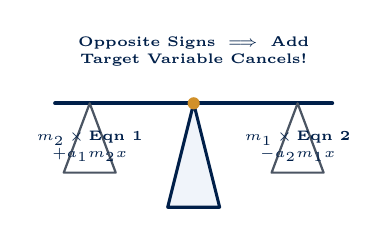
\begin{tikzpicture}[scale=1.1, line cap=round, line join=round]
  % Balance scale
  \draw[primary, line width=1.4pt] (0,0) -- (3.2,0);
  \draw[primary, fill=primarylight, line width=1.1pt] (1.6,0) -- (1.3,-1.2) -- (1.9,-1.2) -- cycle;
  \fill[accent] (1.6,0) circle (2pt);

  % Left Pan
  \draw[secondary, line width=0.8pt] (0.4,0) -- (0.1,-0.8) -- (0.7,-0.8) -- cycle;
  \node[font=\tiny\bfseries\color{navy}, align=center] at (0.4,-0.5) {$m_2 \times \text{Eqn 1}$\\$+a_1 m_2 x$};

  % Right Pan
  \draw[secondary, line width=0.8pt] (2.8,0) -- (2.5,-0.8) -- (3.1,-0.8) -- cycle;
  \node[font=\tiny\bfseries\color{navy}, align=center] at (2.8,-0.5) {$m_1 \times \text{Eqn 2}$\\$-a_2 m_1 x$};

  \node[font=\tiny\bfseries\color{reddeep}, align=center] at (1.6,0.6) {Opposite Signs $\implies$ Add\\Target Variable Cancels!};
\end{tikzpicture}
\end{minipage}

\vspace{0.8mm}
\begin{conceptBox}[title={Worked Archetype 5 $\vert$ NCERT Ratio Income / Expenditure Classic},fonttitle=\bfseries\color{navy}]
  \textbf{Problem:} The ratio of incomes of two persons is $9 : 7$ and the ratio of their expenditures is $4 : 3$. If each of them manages to save \textcurrency$2000\text{ per month}$, find their monthly incomes.
  \par\vspace{0.6mm}\noindent
  \textbf{Step 1: Algebraic Formulation:}\\
  Let their monthly incomes be $9x$ and $7x$, and their monthly expenditures be $4y$ and $3y$.
  $$\text{Income} - \text{Expenditure} = \text{Savings}$$
  $$9x - 4y = 2000 \quad \text{--- (1)}$$
  $$7x - 3y = 2000 \quad \text{--- (2)}$$
  \textbf{Step 2: Eliminate variable $y$ using LCM of coefficients ($4$ and $3 \implies \text{LCM} = 12$):}\\
  Multiply Equation (1) by $3$:
  $$3(9x - 4y) = 3(2000) \implies 27x - 12y = 6000 \quad \text{--- (3)}$$
  Multiply Equation (2) by $4$:
  $$4(7x - 3y) = 4(2000) \implies 28x - 12y = 8000 \quad \text{--- (4)}$$
  \textbf{Step 3: Subtract Equation (3) from Equation (4) (Same signs on $-12y$):}
  $$(28x - 12y) - (27x - 12y) = 8000 - 6000$$
  $$28x - 27x - 12y + 12y = 2000 \implies \mathbf{x = 2000}$$
  \textbf{Step 4: Compute monthly incomes:}
  $$\text{Income of Person 1} = 9x = 9 \times 2000 = \text{\textcurrency}\mathbf{18{,}000}$$
  $$\text{Income of Person 2} = 7x = 7 \times 2000 = \text{\textcurrency}\mathbf{14{,}000}$$
\end{conceptBox}

\newpage

% =============================================================================
% PAGE 7: MODULE 6 — THE SYMMETRIC COEFFICIENTS SYSTEM
% =============================================================================
\thispagestyle{fancy}
\vspace*{0mm}

\chapterbanner{03}{PAIR OF LINEAR EQUATIONS IN TWO VARIABLES}{Module 6 $\vert$ The Symmetric Coefficients Addition/Subtraction Shortcut}{\CoreTag}

\subhead{6.1 Structural Anatomy of Interchanged Coefficients Systems}

When linear systems feature large numerical coefficients where the **coefficients of $x$ and $y$ are interchanged**:
$$\mathbf{ax + by = c} \qquad \text{and} \qquad \mathbf{bx + ay = d}$$
Standard elimination requires calculating huge LCMs (e.g., $152 \times 378$), which leads to massive arithmetic blunders. The **Maths Manthan 2-Step Addition/Subtraction Shortcut** reduces the system to mental arithmetic!

\begin{center}
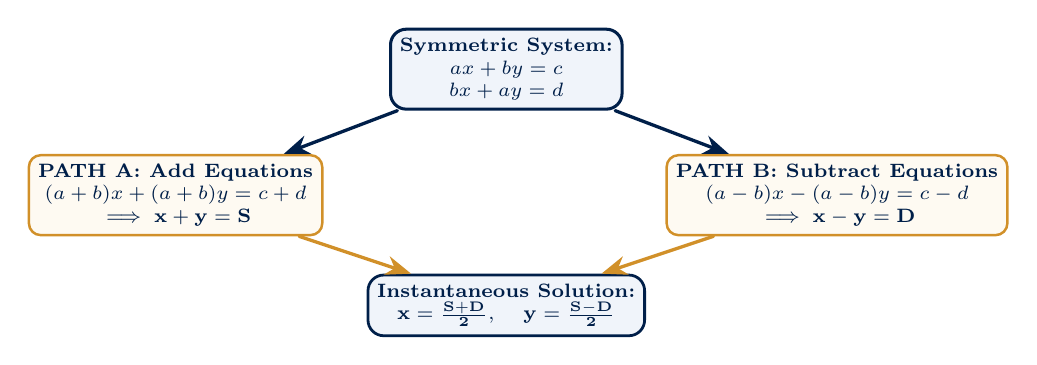
\begin{tikzpicture}[scale=1.0, line cap=round, line join=round]
  % Center System
  \node[draw=primary, fill=primarylight, rounded corners=2mm, line width=1.1pt, font=\scriptsize\bfseries\color{navy}, align=center] (SYS) at (0,2.4) {Symmetric System:\\$ax + by = c$\\$bx + ay = d$};

  % Left branch: ADD
  \node[draw=accent, fill=accentlight, rounded corners=1.5mm, line width=0.9pt, font=\scriptsize\bfseries\color{navy}, align=center] (ADD) at (-4.2,0.8) {PATH A: Add Equations\\$(a+b)x + (a+b)y = c+d$\\$\implies \mathbf{x + y = S}$};

  % Right branch: SUBTRACT
  \node[draw=accent, fill=accentlight, rounded corners=1.5mm, line width=0.9pt, font=\scriptsize\bfseries\color{navy}, align=center] (SUB) at (4.2,0.8) {PATH B: Subtract Equations\\$(a-b)x - (a-b)y = c-d$\\$\implies \mathbf{x - y = D}$};

  % Final Solution
  \node[draw=green, fill=greenpale, rounded corners=2mm, line width=1pt, font=\scriptsize\bfseries\color{green}, align=center] (SOL) at (0,-0.6) {Instantaneous Solution:\\$\mathbf{x = \frac{S + D}{2}}, \quad \mathbf{y = \frac{S - D}{2}}$};

  \draw[-{Stealth[scale=1.1]}, primary, line width=1.2pt] (SYS) -- (ADD);
  \draw[-{Stealth[scale=1.1]}, primary, line width=1.2pt] (SYS) -- (SUB);
  \draw[-{Stealth[scale=1.1]}, accent, line width=1.2pt] (ADD) -- (SOL);
  \draw[-{Stealth[scale=1.1]}, accent, line width=1.2pt] (SUB) -- (SOL);
\end{tikzpicture}
\end{center}

\vspace{0.8mm}
\begin{conceptBox}[title={Worked Archetype 6 $\vert$ High-Speed Solution of Large Symmetric Coefficients},fonttitle=\bfseries\color{navy}]
  \textbf{Problem:} Solve the following pair of equations:
  $$152x - 378y = -74 \quad \text{--- (1)} \qquad \text{and} \qquad -378x + 152y = -604 \quad \text{--- (2)}$$
  \par\vspace{0.6mm}\noindent
  \textbf{Step 1: Add Equation (1) and Equation (2):}
  $$(152 - 378)x + (-378 + 152)y = -74 - 604$$
  $$-226x - 226y = -678$$
  Divide through by $-226$:
  $$\mathbf{x + y = 3} \quad \text{--- (3)}$$
  \textbf{Step 2: Subtract Equation (2) from Equation (1):}
  $$[152 - (-378)]x + [-378 - 152]y = -74 - (-604)$$
  $$530x - 530y = 530$$
  Divide through by $530$:
  $$\mathbf{x - y = 1} \quad \text{--- (4)}$$
  \textbf{Step 3: Solve the simplified system of Equations (3) and (4):}
  $$\text{Add (3) and (4): } 2x = 4 \implies \mathbf{x = 2}$$
  $$\text{Subtract (4) from (3): } 2y = 2 \implies \mathbf{y = 1}$$
  \textbf{Conclusion:} The solution is $\mathbf{x = 2, \; y = 1}$. (Solved in 30 seconds without large multiplications!).
\end{conceptBox}

\newpage

% =============================================================================
% PAGE 8: MODULE 7 — CONSISTENCY & PARAMETER k PROTOCOLS
% =============================================================================
\thispagestyle{fancy}
\vspace*{0mm}

\chapterbanner{03}{PAIR OF LINEAR EQUATIONS IN TWO VARIABLES}{Module 7 $\vert$ Consistency Conditions \& The Parameter $k$ Protocols}{\CoreTag}

\subhead{7.1 Rigorous Protocol for Parameter $k$ Determination}

A very high-frequency question in CBSE board examinations asks for values of $k$ satisfying a given consistency condition:

\begin{center}
\small
\begin{tabularx}{\textwidth}{p{32mm} c p{38mm} X}
\toprule
\rowcolor{bluepale}
\textbf{Specified Condition} & \textbf{Algebraic Ratio Equation} & \textbf{Solving Protocol} & \textbf{Mandatory Verification Check} \\
\midrule
\textbf{Unique Solution} & $\frac{a_1}{a_2} \neq \frac{b_1}{b_2}$ & Solve $a_1 b_2 - a_2 b_1 \neq 0$ & State: "$k$ can be \textbf{any real number except} $k_0$". \\
\rowcolor{lightgray}
\textbf{Infinitely Many} & $\frac{a_1}{a_2} = \frac{b_1}{b_2} = \frac{c_1}{c_2}$ & Equate Pair 1 ($\frac{a_1}{a_2}=\frac{b_1}{b_2}$) AND Pair 2 ($\frac{b_1}{b_2}=\frac{c_1}{c_2}$) & \textbf{\TrapTag\ Both pairs must yield the SAME value of $k$}! \\
\textbf{No Solution} & $\frac{a_1}{a_2} = \frac{b_1}{b_2} \neq \frac{c_1}{c_2}$ & Equate $\frac{a_1}{a_2}=\frac{b_1}{b_2}$ and verify $\neq \frac{c_1}{c_2}$ & Reject any candidate $k$ that makes $\frac{b_1}{b_2} = \frac{c_1}{c_2}$. \\
\bottomrule
\end{tabularx}
\end{center}

\vspace{0.8mm}
\begin{conceptBox}[title={Worked Archetype 7 $\vert$ The Dual-Pair Consistency Trap in Infinite Solutions},fonttitle=\bfseries\color{navy}]
  \textbf{Problem:} Find the value(s) of $k$ for which the following pair of linear equations has infinitely many solutions:
  $$kx + 3y - (k - 3) = 0 \qquad \text{and} \qquad 12x + ky - k = 0$$
  \par\vspace{0.6mm}\noindent
  \textbf{Step 1: Identify coefficients in standard form:}
  $$a_1 = k, \; b_1 = 3, \; c_1 = -(k - 3) \qquad \text{and} \qquad a_2 = 12, \; b_2 = k, \; c_2 = -k$$
  \textbf{Step 2: Set up the condition for infinitely many solutions:}
  $$\frac{a_1}{a_2} = \frac{b_1}{b_2} = \frac{c_1}{c_2} \implies \frac{k}{12} = \frac{3}{k} = \frac{-(k - 3)}{-k} = \frac{k - 3}{k}$$
  \textbf{Step 3: Solve the first pair of ratios:}
  $$\frac{k}{12} = \frac{3}{k} \implies k^2 = 36 \implies \mathbf{k = \pm 6} \implies k = 6 \quad \text{or} \quad k = -6$$
  \textbf{\TrapTag\ Critical Board Examination Audit:} Do NOT stop here! You must verify which sign satisfies the second ratio:
  $$\frac{3}{k} = \frac{k - 3}{k}$$
  Cross-multiplying (for $k \neq 0$):
  $$3k = k(k - 3) \implies 3 = k - 3 \implies \mathbf{k = 6}$$
  \textbf{Step 4: Check consistency for $k = -6$:}
  $$\text{For } k = -6: \quad \frac{a_1}{a_2} = \frac{-6}{12} = -\frac{1}{2}, \quad \frac{b_1}{b_2} = \frac{3}{-6} = -\frac{1}{2}, \quad \frac{c_1}{c_2} = \frac{-6 - 3}{-6} = \frac{-9}{-6} = \frac{3}{2}$$
  Here $\frac{a_1}{a_2} = \frac{b_1}{b_2} \neq \frac{c_1}{c_2}$, which gives \textbf{no solution}, NOT infinitely many!\\
  Hence, $\mathbf{k = -6}$ is \textbf{strictly rejected}.\\
  \textbf{Conclusion:} The only value of $k$ for which the system has infinitely many solutions is $\mathbf{k = 6}$.
\end{conceptBox}

\newpage

% =============================================================================
% PAGE 9: MODULE 8 — WORD PROBLEMS I: NUMBERS, DIGITS & FRACTIONS
% =============================================================================
\thispagestyle{fancy}
\vspace*{0mm}

\chapterbanner{03}{PAIR OF LINEAR EQUATIONS IN TWO VARIABLES}{Module 8 $\vert$ Word Problems I: Numbers, 2-Digit Reversals \& Fractions}{\CoreTag}

\subhead{8.1 The Two-Digit Number Decimal Place Value Model}

A two-digit number cannot be written as $xy$ (which represents a product!). In our base-10 positional numeral system:
\begin{formulaBox}
  $$\mathbf{\text{Original Two-Digit Number}} = \mathbf{10x + y} \quad (\text{where } x = \text{tens digit}, \; y = \text{units digit})$$
  $$\mathbf{\text{Reversed Two-Digit Number}} = \mathbf{10y + x}$$
  \textbf{Universal Algebraic Properties:}
  \begin{itemize}
    \item \textbf{Sum of Number and its Reverse:} $(10x + y) + (10y + x) = 11x + 11y = \mathbf{11(x + y)}$ (\textit{always a multiple of 11!})
    \item \textbf{Difference of Number and its Reverse:} $(10x + y) - (10y + x) = 9x - 9y = \mathbf{9(x - y)}$ (\textit{always a multiple of 9!})
  \end{itemize}
\end{formulaBox}

\vspace{0.8mm}
\subhead{8.2 Fraction Modification Models}

Let the original fraction be $\mathbf{\frac{x}{y}}$ (where $x = \text{numerator}, y = \text{denominator}, y \neq 0$):
\begin{itemize}
  \item If $c$ is added to both numerator and denominator: $\frac{x + c}{y + c} = \frac{p}{q} \implies q(x + c) = p(y + c)$.
\end{itemize}

\vspace{0.8mm}
\begin{conceptBox}[title={Worked Archetype 8 $\vert$ Reversible Two-Digit Number Problem},fonttitle=\bfseries\color{navy}]
  \textbf{Problem:} The sum of a two-digit number and the number obtained by reversing the digits is $66$. If the digits of the number differ by $2$, find the number. How many such numbers are there?
  \par\vspace{0.6mm}\noindent
  \textbf{Step 1: Set up variables:} Let the tens digit be $x$ and the units digit be $y$.\\
  $\text{Original Number} = 10x + y$, \quad $\text{Reversed Number} = 10y + x$.
  \par\noindent
  \textbf{Step 2: First condition (Sum is 66):}
  $$(10x + y) + (10y + x) = 66 \implies 11x + 11y = 66 \implies \mathbf{x + y = 6} \quad \text{--- (1)}$$
  \textbf{Step 3: Second condition (Digits differ by 2):}
  Since it is not specified whether $x > y$ or $y > x$, we have two cases:
  $$\mathbf{x - y = 2} \quad \text{--- (2a)} \qquad \text{or} \qquad \mathbf{y - x = 2} \quad \text{--- (2b)}$$
  \textbf{Step 4: Solve Case A: Equations (1) and (2a):}
  $$\text{Adding (1) and (2a): } 2x = 8 \implies x = 4 \implies y = 6 - 4 = 2$$
  $$\text{Number} = 10(4) + 2 = \mathbf{42}$$
  \textbf{Step 5: Solve Case B: Equations (1) and (2b):}
  $$\text{Adding (1) and (2b): } 2y = 8 \implies y = 4 \implies x = 6 - 4 = 2$$
  $$\text{Number} = 10(2) + 4 = \mathbf{24}$$
  \textbf{Conclusion:} There are \textbf{two such numbers}: $\mathbf{42}$ and $\mathbf{24}$.
\end{conceptBox}

\newpage

% =============================================================================
% PAGE 10: MODULE 9 — WORD PROBLEMS II: AGES & GEOMETRY
% =============================================================================
\thispagestyle{fancy}
\vspace*{0mm}

\chapterbanner{03}{PAIR OF LINEAR EQUATIONS IN TWO VARIABLES}{Module 9 $\vert$ Word Problems II: Age Relations \& Geometry / Cyclic Quadrilaterals}{\CoreTag}

\subhead{10.1 Age Relationship Dynamics: Past vs. Future}

Let present ages of two individuals $A$ and $B$ be $x$ and $y$ years:
\begin{itemize}
  \item \textbf{$n$ Years Ago (Past):} Both ages decrease equally: $\mathbf{(x - n)}$ and $\mathbf{(y - n)}$.
  \item \textbf{$m$ Years Hence (Future):} Both ages increase equally: $\mathbf{(x + m)}$ and $\mathbf{(y + m)}$.
\end{itemize}

\vspace{0.8mm}
\subhead{10.2 Geometric Angle Systems \& Cyclic Quadrilaterals}

\begin{minipage}[c]{0.45\textwidth}
\centering
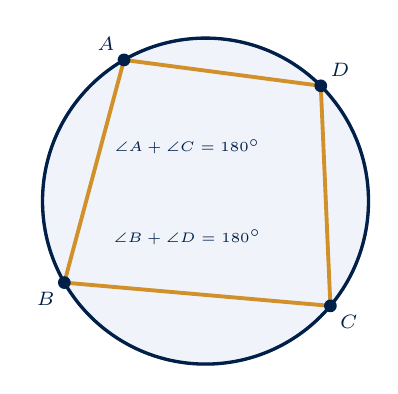
\begin{tikzpicture}[scale=1.15, line cap=round, line join=round]
  % Circle
  \draw[primary!30, fill=primarylight, line width=1pt] (0,0) circle (1.8cm);
  \draw[primary, line width=1.2pt] (0,0) circle (1.8cm);

  % Quadrilateral vertices
  \coordinate (A) at ({1.8*cos(120)},{1.8*sin(120)});
  \coordinate (B) at ({1.8*cos(210)},{1.8*sin(210)});
  \coordinate (C) at ({1.8*cos(320)},{1.8*sin(320)});
  \coordinate (D) at ({1.8*cos(45)},{1.8*sin(45)});

  \draw[accent, line width=1.4pt] (A) -- (B) -- (C) -- (D) -- cycle;

  \fill[reddeep] (A) circle (2pt) node[above left, font=\scriptsize\bfseries\color{reddeep}]{$A$};
  \fill[primary] (B) circle (2pt) node[below left, font=\scriptsize\bfseries\color{navy}]{$B$};
  \fill[reddeep] (C) circle (2pt) node[below right, font=\scriptsize\bfseries\color{reddeep}]{$C$};
  \fill[primary] (D) circle (2pt) node[above right, font=\scriptsize\bfseries\color{navy}]{$D$};

  \node[font=\tiny\bfseries\color{reddeep}] at (-0.2,0.6) {$\angle A + \angle C = 180^\circ$};
  \node[font=\tiny\bfseries\color{navy}] at (-0.2,-0.4) {$\angle B + \angle D = 180^\circ$};
\end{tikzpicture}
\end{minipage}\hfill
\begin{minipage}[c]{0.53\textwidth}
\begin{formulaBox}
  \textbf{Cyclic Quadrilateral Theorem:}
  A quadrilateral $ABCD$ is cyclic (all 4 vertices lie on a circle) if and only if its \textbf{opposite angles are supplementary}:
  $$\mathbf{\angle A + \angle C = 180^\circ}$$
  $$\mathbf{\angle B + \angle D = 180^\circ}$$
  This immediately sets up a decoupled pair of linear equations in $x$ and $y$!
\end{formulaBox}
\end{minipage}

\vspace{0.8mm}
\begin{conceptBox}[title={Worked Archetype 9 $\vert$ The Angles of a Cyclic Quadrilateral},fonttitle=\bfseries\color{navy}]
  \textbf{Problem:} $ABCD$ is a cyclic quadrilateral. Find the angles of the cyclic quadrilateral if:
  $$\angle A = 4y + 20, \quad \angle B = 3y - 5, \quad \angle C = -4x, \quad \angle D = -7x + 5$$
  \par\vspace{0.6mm}\noindent
  \textbf{Step 1: Set up Equation 1 using opposite angles $A$ and $C$:}
  $$\angle A + \angle C = 180^\circ \implies (4y + 20) + (-4x) = 180^\circ$$
  $$-4x + 4y = 160 \implies \text{Divide by } -4: \quad \mathbf{x - y = -40} \quad \text{--- (1)}$$
  \textbf{Step 2: Set up Equation 2 using opposite angles $B$ and $D$:}
  $$\angle B + \angle D = 180^\circ \implies (3y - 5) + (-7x + 5) = 180^\circ$$
  $$-7x + 3y = 180 \quad \text{--- (2)}$$
  \textbf{Step 3: Solve the system using substitution $x = y - 40$ from (1) into (2):}
  $$-7(y - 40) + 3y = 180 \implies -7y + 280 + 3y = 180$$
  $$-4y = 180 - 280 = -100 \implies \mathbf{y = 25}$$
  $$x = y - 40 = 25 - 40 \implies \mathbf{x = -15}$$
  \textbf{Step 4: Compute the four angles:}
  $$\angle A = 4(25) + 20 = 100 + 20 = \mathbf{120^\circ}$$
  $$\angle B = 3(25) - 5 = 75 - 5 = \mathbf{70^\circ}$$
  $$\angle C = -4(-15) = \mathbf{60^\circ}$$
  $$\angle D = -7(-15) + 5 = 105 + 5 = \mathbf{110^\circ}$$
  \textbf{Check:} $\angle A + \angle C = 120^\circ + 60^\circ = 180^\circ$, and $\angle B + \angle D = 70^\circ + 110^\circ = 180^\circ$.
\end{conceptBox}

\newpage

% =============================================================================
% PAGE 11: MODULE 10 — WORD PROBLEMS III: CHARGES & SPEED
% =============================================================================
\thispagestyle{fancy}
\vspace*{0mm}

\chapterbanner{03}{PAIR OF LINEAR EQUATIONS IN TWO VARIABLES}{Module 10 $\vert$ Word Problems III: Fixed Charges \& Relative Speed Kinematics}{\CoreTag}

\subhead{11.1 The Fixed Charge Plus Variable Rate Model}

Common real-world models (taxis, library lending, hostel boarding) feature a two-part cost structure:
\begin{formulaBox}
  $$\mathbf{\text{Total Charge } C(d) = \text{Fixed Base Charge } (x) + (\text{Distance / Days } d) \times \text{Rate per unit } (y)}$$
  $$\mathbf{x + d_1 y = C_1} \qquad \text{and} \qquad \mathbf{x + d_2 y = C_2}$$
  \textit{Subtracting Equation 1 from Equation 2 immediately eliminates the fixed charge $x$!}
\end{formulaBox}

\begin{minipage}[c]{0.45\textwidth}
\centering
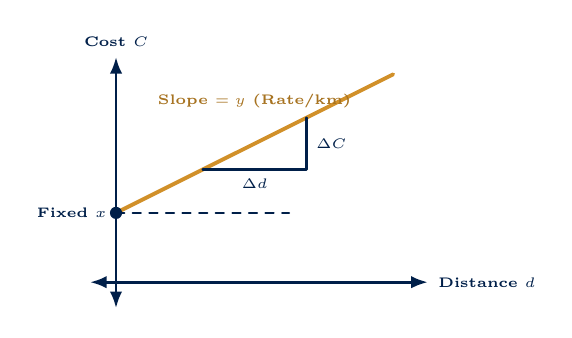
\begin{tikzpicture}[scale=1.1, line cap=round, line join=round]
  % Axes
  \draw[{Latex[scale=0.8]}-{Latex[scale=0.8]}, primary, line width=1pt] (-0.3,0) -- (3.6,0) node[right, font=\tiny\bfseries]{Distance $d$};
  \draw[{Latex[scale=0.8]}-{Latex[scale=0.8]}, primary, line width=1pt] (0,-0.3) -- (0,2.6) node[above, font=\tiny\bfseries]{Cost $C$};

  % Linear function
  \draw[accent, line width=1.4pt] (0,0.8) -- (3.2,2.4);

  % Intercept
  \fill[reddeep] (0,0.8) circle (2pt) node[left, font=\tiny\bfseries\color{reddeep}]{Fixed $x$};
  \draw[dashed, reddeep, line width=0.7pt] (0,0.8) -- (2.0,0.8);

  % Slope triangle
  \draw[primary, line width=0.8pt] (1.0,1.3) -- (2.2,1.3) -- (2.2,1.9);
  \node[font=\tiny\bfseries\color{primary}, below] at (1.6,1.3) {$\Delta d$};
  \node[font=\tiny\bfseries\color{primary}, right] at (2.2,1.6) {$\Delta C$};
  \node[font=\tiny\bfseries\color{accent!80!black}, above] at (1.6,1.9) {Slope $= y$ (Rate/km)};
\end{tikzpicture}
\end{minipage}\hfill
\begin{minipage}[c]{0.53\textwidth}
\begin{formulaBox}
  \textbf{Relative Highway Speeds (Cars A and B):}
  Let car from A have speed $x\text{ km/h}$, car from B have speed $y\text{ km/h}$ ($x > y$), distance $D$:
  \begin{itemize}
    \item \textbf{Same Direction:} Relative speed $= \mathbf{x - y}$.
      $$(x - y) \cdot t_{\text{same}} = D$$
    \item \textbf{Opposite Directions (Towards each other):} Relative speed $= \mathbf{x + y}$.
      $$(x + y) \cdot t_{\text{opp}} = D$$
  \end{itemize}
\end{formulaBox}
\end{minipage}

\vspace{0.8mm}
\begin{conceptBox}[title={Worked Archetype 10 $\vert$ Taxi Cab Fixed and Distance Charges},fonttitle=\bfseries\color{navy}]
  \textbf{Problem:} The taxi charges in a city consist of a fixed charge together with the charge for the distance covered. For a distance of $10\text{ km}$, the charge paid is \textcurrency$105$ and for a journey of $15\text{ km}$, the charge paid is \textcurrency$155$. What are the fixed charges and the charge per km? How much does a person have to pay for travelling a distance of $25\text{ km}$?
  \par\vspace{0.6mm}\noindent
  \textbf{Step 1: Formulate linear equations:}\\
  Let fixed charge $= \text{\textcurrency}x$, and charge per km $= \text{\textcurrency}y$.
  $$x + 10y = 105 \quad \text{--- (1)}$$
  $$x + 15y = 155 \quad \text{--- (2)}$$
  \textbf{Step 2: Subtract Equation (1) from Equation (2):}
  $$(x + 15y) - (x + 10y) = 155 - 105 \implies 5y = 50 \implies \mathbf{y = 10}$$
  \textbf{Step 3: Substitute $y = 10$ into Equation (1):}
  $$x + 10(10) = 105 \implies x + 100 = 105 \implies \mathbf{x = 5}$$
  $$\mathbf{\text{Fixed Charge} = \text{\textcurrency}5}, \qquad \mathbf{\text{Charge per km} = \text{\textcurrency}10}$$
  \textbf{Step 4: Compute charge for $25\text{ km}$:}
  $$\text{Total Cost} = x + 25y = 5 + 25(10) = 5 + 250 = \text{\textcurrency}\mathbf{255}$$
\end{conceptBox}

\newpage

% =============================================================================
% PAGE 12: MODULE 11 — MASTER FORMULA MATRIX & DECISION TREE
% =============================================================================
\thispagestyle{fancy}
\vspace*{0mm}

\chapterbanner{03}{PAIR OF LINEAR EQUATIONS IN TWO VARIABLES}{Module 11 $\vert$ Master Formula Matrix \& Solution Decision Protocol}{\ReferenceTag}

\subhead{11.1 The Comprehensive Linear Systems Matrix}

\begin{center}
\small
\begin{tabularx}{\textwidth}{>{\bfseries}p{30mm} c p{38mm} X}
\toprule
\rowcolor{bluepale}
Method / Criterion & Prerequisite Form & Mathematical Rule & Strategic Board Examination Purpose \\
\midrule
Ratio Test & Standard form & $\frac{a_1}{a_2} \text{ vs } \frac{b_1}{b_2} \text{ vs } \frac{c_1}{c_2}$ & Pre-test consistency before solving. \\
\rowcolor{lightgray}
Graphical Method & Table of values & Intersection $(x_0, y_0)$ & Visual proof; finding bounded triangle area. \\
Substitution & Isolate 1 variable & $x = f(y) \implies a_2 f(y) + b_2 y = c_2$ & Best when a variable has coefficient $\pm 1$. \\
\rowcolor{lightgray}
Elimination & Equalize coefficients & Add if diff signs, Sub if same & Fastest general method for non-unit coefficients. \\
Symmetric Shortcut & $ax+by=c, bx+ay=d$ & Add for $x+y$, Sub for $x-y$ & Eliminates huge multi-digit LCM calculations. \\
\rowcolor{lightgray}
Triangle with $x$-axis & Intersecting lines & Vertices $P(x_0, y_0), A, B$ & $\text{Area} = \frac{1}{2} \cdot |x_B - x_A| \cdot |y_0|$. \\
Number Reversal & 2-digit number & $10x + y \leftrightarrow 10y + x$ & Sum is $11(x+y)$; Difference is $9(x-y)$. \\
\bottomrule
\end{tabularx}
\end{center}

\vspace{0.8mm}
\subhead{11.2 The 3-Tier Linear System Decision Flowchart}

\begin{center}
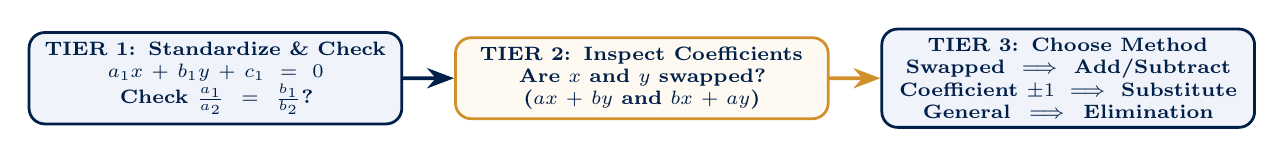
\begin{tikzpicture}[scale=0.95, line cap=round, line join=round]
  % Step 1
  \node[draw=primary, fill=primarylight, rounded corners=2mm, line width=1pt, font=\scriptsize\bfseries\color{navy}, align=center, text width=4.5cm] (Q1) at (0,2.5) {TIER 1: Standardize \& Check\\$a_1 x + b_1 y + c_1 = 0$\\Check $\frac{a_1}{a_2} = \frac{b_1}{b_2}$?};

  % Step 2
  \node[draw=accent, fill=accentlight, rounded corners=2mm, line width=1pt, font=\scriptsize\bfseries\color{navy}, align=center, text width=4.5cm] (Q2) at (5.7,2.5) {TIER 2: Inspect Coefficients\\Are $x$ and $y$ swapped?\\($ax+by$ and $bx+ay$)};

  % Step 3
  \node[draw=primary, fill=primarylight, rounded corners=2mm, line width=1pt, font=\scriptsize\bfseries\color{navy}, align=center, text width=4.5cm] (Q3) at (11.4,2.5) {TIER 3: Choose Method\\Swapped $\implies$ Add/Subtract\\Coefficient $\pm 1 \implies$ Substitute\\General $\implies$ Elimination};

  \draw[-{Stealth[scale=1.1]}, primary, line width=1.3pt] (Q1) -- (Q2);
  \draw[-{Stealth[scale=1.1]}, accent, line width=1.3pt] (Q2) -- (Q3);
\end{tikzpicture}
\end{center}

\vspace{0.8mm}
\begin{formulaBox}
  \textbf{Strategic Rules for Method Selection:}
  \begin{itemize}
    \item \textbf{Use Substitution when:} At least one variable in either equation has coefficient $+1$ or $-1$ (e.g., $x + 2y = 3$).
    \item \textbf{Use Elimination when:} All coefficients are $> 1$ and non-symmetric (e.g., $9x - 4y = 2000$ and $7x - 3y = 2000$).
    \item \textbf{Use Add/Subtract Shortcut when:} Coefficients are large and interchanged ($152x - 378y$ and $-378x + 152y$).
  \end{itemize}
\end{formulaBox}

\newpage

% =============================================================================
% PAGE 13: MODULE 12 — BOARD EXAM CASE-STUDY & CONTEXTUAL MODELING
% =============================================================================
\thispagestyle{fancy}
\vspace*{0mm}

\chapterbanner{03}{PAIR OF LINEAR EQUATIONS IN TWO VARIABLES}{Module 12 $\vert$ Applied Case-Study: Urban Transport \& Electric Cab Pricing}{\ExamTag}

\subhead{Case Study 1 $\vert$ Eco-Transit Smart Mobility Fare Structure}

A metropolitan city introduces an electric green-cab service. The pricing policy consists of a minimum initial boarding fee (fixed charge) plus a constant variable rate per kilometer.
\begin{itemize}
  \item Aditi travels $12\text{ km}$ from the railway station to her office and pays \textcurrency$145$.
  \item Rahul travels $18\text{ km}$ across the city for a business summit and pays \textcurrency$205$.
\end{itemize}

\begin{minipage}[c]{0.42\textwidth}
\centering
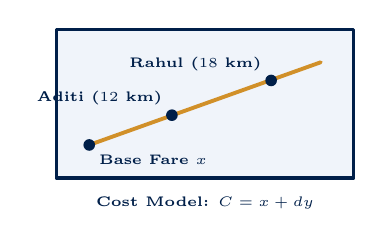
\begin{tikzpicture}[scale=1.05, line cap=round, line join=round]
  % Graphic of cab / distance
  \draw[primary, fill=primarylight, line width=1.1pt] (-0.2,0) rectangle (3.4,1.8);

  \draw[accent, line width=1.4pt] (0.2,0.4) -- (3.0,1.4);
  \fill[reddeep] (0.2,0.4) circle (2pt) node[below right, font=\tiny\bfseries\color{reddeep}]{Base Fare $x$};

  \fill[primary] (1.2,0.76) circle (2pt) node[above left, font=\tiny\bfseries]{Aditi ($12\text{ km}$)};
  \fill[primary] (2.4,1.18) circle (2pt) node[above left, font=\tiny\bfseries]{Rahul ($18\text{ km}$)};

  \node[font=\tiny\bfseries\color{navy}, align=center] at (1.6,-0.3) {Cost Model: $C = x + dy$};
\end{tikzpicture}
\end{minipage}\hfill
\begin{minipage}[c]{0.56\textwidth}
\begin{conceptBox}[title={4-Mark Board Question Protocol},fonttitle=\bfseries\color{navy}]
  \textbf{Questions:}
  \begin{enumerate}
    \item Represent the given information algebraically as a pair of linear equations in two variables. [1M]
    \item Find the fixed charge and the charge per kilometer. [2M]
    \item How much will a commuter pay for a journey of $30\text{ km}$? [1M]
  \end{enumerate}
\end{conceptBox}
\end{minipage}

\vspace{0.8mm}
\begin{successBox}[title={Solution \& Marking Scheme Evaluation},fonttitle=\bfseries\color{navy}]
  \begin{enumerate}
    \item \textbf{Algebraic Formulation [1M]:} Let fixed boarding charge $= \text{\textcurrency}x$, and rate per km $= \text{\textcurrency}y$.
      $$x + 12y = 145 \quad \text{--- (1)}$$
      $$x + 18y = 205 \quad \text{--- (2)}$$
    \item \textbf{Solving for $x$ and $y$ [2M]:}
      Subtract Equation (1) from Equation (2):
      $$(x + 18y) - (x + 12y) = 205 - 145$$
      $$6y = 60 \implies \mathbf{y = 10\text{ \textcurrency/km}}$$
      Substitute $y = 10$ into Equation (1):
      $$x + 12(10) = 145 \implies x + 120 = 145 \implies \mathbf{x = 25\text{ \textcurrency}}$$
      \textbf{Answer:} Fixed charge is $\mathbf{\text{\textcurrency}25}$, and charge per km is $\mathbf{\text{\textcurrency}10}$.
    \item \textbf{Fare for $30\text{ km}$ Journey [1M]:}
      $$\text{Total Fare} = x + 30y = 25 + 30(10) = 25 + 300 = \text{\textcurrency}\mathbf{325}$$
  \end{enumerate}
\end{successBox}

\newpage

% =============================================================================
% PAGE 14: MODULE 13 — CBSE BOARD TRAPS, HACKS & PRE-SUBMISSION AUDIT
% =============================================================================
\thispagestyle{fancy}
\vspace*{0mm}

\chapterbanner{03}{PAIR OF LINEAR EQUATIONS IN TWO VARIABLES}{Module 13 $\vert$ Board Traps, Verification Hacks \& 5-Point Audit}{\ExamTag}

\subhead{13.1 The Top 7 Linear Equation Board Traps (And How to Bust Them)}

\begin{enumerate}[label=\textbf{Trap \arabic*:}, leftmargin=5mm, itemsep=1pt, topsep=0.8pt, parsep=0pt]
  \item \textbf{The Constant Term Position Asymmetry Trap:} Comparing $\frac{c_1}{c_2}$ when one equation has constant on LHS and other on RHS (e.g., $2x + 3y = 7$ and $4x + 6y - 14 = 0$). \TrapTag\ You must move both constants to the \textbf{same side} before taking ratios!
  \item \textbf{The Missing Sign in Subtraction of Equations:} In elimination, when subtracting $(-3y)$ from $(-5y)$, mistakenly writing $-8y$ instead of $-5y - (-3y) = \mathbf{-2y}$.
  \item \textbf{The Incomplete Parameter $k$ Check:} In infinite solutions, taking only $\frac{a_1}{a_2} = \frac{b_1}{b_2}$ and forgetting to check $\frac{b_1}{b_2} = \frac{c_1}{c_2}$. A single equation cannot confirm infinite solutions!
  \item \textbf{The Two-Digit Number Variable Trap:} Writing the two-digit number as $xy$ or $x + y$. The decimal number is strictly $\mathbf{10x + y}$.
  \item \textbf{Shading the Wrong Triangular Region:} Shading the triangle formed with the $y$-axis when the question asks for the triangle formed with the \textbf{$x$-axis}. Always highlight the specified axis first!
  \item \textbf{Inverting Relative Speed in Rivers:} Writing upstream speed as $y - x$. The boat speed must exceed stream speed, so upstream is strictly $\mathbf{x - y}$.
  \item \textbf{Using the Deleted Cross-Multiplication Method:} The cross-multiplication formula is deleted from the CBSE curriculum. Solve strictly using \textbf{Substitution} or \textbf{Elimination}.
\end{enumerate}

\subhead{13.2 High-Speed Algebraic Verification Protocol}

Before turning in your answer sheet, always substitute your computed values of $(x, y)$ into \textbf{both original equations}:
$$\text{Check 1: } a_1 x_0 + b_1 y_0 + c_1 \stackrel{?}{=} 0 \qquad \text{and} \qquad \text{Check 2: } a_2 x_0 + b_2 y_0 + c_2 \stackrel{?}{=} 0$$
If it satisfies both, your solution is $100\%$ mathematically guaranteed!

\vspace{1mm}
\subhead{13.3 The 5-Point Board Examination Pre-Submission Checklist}

\begin{successBox}[top=1.2mm,bottom=1.2mm,before skip=1.5pt,after skip=1pt]
  \textbf{Final 60-Second Answer Sheet Verification Protocol:}
  \begin{itemize}[leftmargin=4mm,itemsep=1pt,topsep=1pt,parsep=0pt]
    \item[$\square$] \textbf{Standard Form Alignment:} Were both equations rearranged with constants on the same side before checking ratios?
    \item[$\square$] \textbf{Ratio Comparison Stated:} Did you write $\frac{a_1}{a_2} \neq \frac{b_1}{b_2}$ explicitly before declaring unique solution? (Guarantees method marks).
    \item[$\square$] \textbf{Both Variables Solved:} Did you find both $x$ AND $y$? (Don't leave after finding just one!).
    \item[$\square$] \textbf{Triangle Vertices Explicitly Listed:} In graphical questions, did you write the coordinates of all 3 vertices $(x_1, y_1), (x_2, y_2), (x_3, y_3)$?
    \item[$\square$] \textbf{Units Attached in Word Problems:} Incomes in $\mathbf{\text{\textcurrency}}$, Speeds in $\mathbf{\text{km/h}}$, Ages in $\mathbf{\text{years}}$!
  \end{itemize}
\end{successBox}

\vfill
\begin{center}
  {\footnotesize\bfseries\color{primary}MATHS MANTHAN TUITION CLASSES \quad$\vert$\quad END OF CHAPTER 3 HANDBOOK}\\[1mm]
  {\scriptsize\color{secondary}Designed for Academic Excellence in CBSE Class 10 Board Examinations 2026--27.}
\end{center}

\end{document}
